% !TeX encoding = UTF-8
% !TeX spellcheck = pl_PL
\documentclass{article}
\newcommand\tab[1][1cm]{\hspace*{#1}}
\usepackage[]{polski}
\usepackage[utf8]{inputenc}
\usepackage{graphicx}
\usepackage{float}
\usepackage{amsmath}
\usepackage{geometry}
 
\usepackage{listings}
\usepackage{color}
\usepackage{hyperref}


\usepackage{pdfpages}

\definecolor{codegreen}{rgb}{0,0.6,0}
\definecolor{codegray}{rgb}{0.5,0.5,0.5}
\definecolor{codepurple}{rgb}{0.58,0,0.82}
\definecolor{backcolour}{rgb}{0.95,0.95,0.92}

\lstdefinestyle{mystyle}{
	backgroundcolor=\color{backcolour},   
	commentstyle=\color{black},
	keywordstyle=\color{blue},
	numberstyle=\tiny\color{codegray},
	stringstyle=\color{codepurple},
	basicstyle=\footnotesize,
	breakatwhitespace=false,         
	breaklines=true,                 
	captionpos=b,                    
	keepspaces=true,                 
	%numbers=left,                    
	%numbersep=5pt,                  
	showspaces=false,                
	showstringspaces=false,
	showtabs=false,                  
	tabsize=2
}

\lstset{style=mystyle}
\date{}

\author{Kamila Lis i Karolina Borkwoska}

\title{Wykrywanie nieaktywności routerów w sieci SDN\\
	{\large Dokumentacja wstępna projektu programowalnej sieci komputerowej}}

\begin{document}
	\maketitle
	\section{Treść zadania}
	W projekcie należy zaimplementować wykrywanie nieaktywności routerów znajdujących się w~sieci. Następnie sterownik ma za zadanie dostosować tablice przepływu tak, aby ruch nie odbywał się na uszkodzonej ścieżce.
	\section{Rozwiązanie} 
	Sterownik co 30 sekund (kierując się wytycznymi protokołu RIP) odpytuje połączone z~nim routery co do ich aktywności. W~przypadku jej braku następuje aktualizacja tablic przepływu tak by pakiety poruszały się alternatywną trasą.
	\subsection{Narzędzia}
	Projekt postanowiono przeprowadzić przy wykorzystaniu narzędzi \texttt{Mininet} do symulacji architektury oraz \texttt{POX} do implementacji sterownika. Do wykrywania urządzeń sieciowych w sieci wykorzystano pakiet \texttt{openflow.discovery}.
	\subsection{Architektura rozwiązania}
	Rysunek \ref{f:arch} przedstawia przyjętą architekturę sieci. 
	\begin{figure}
		\centering
		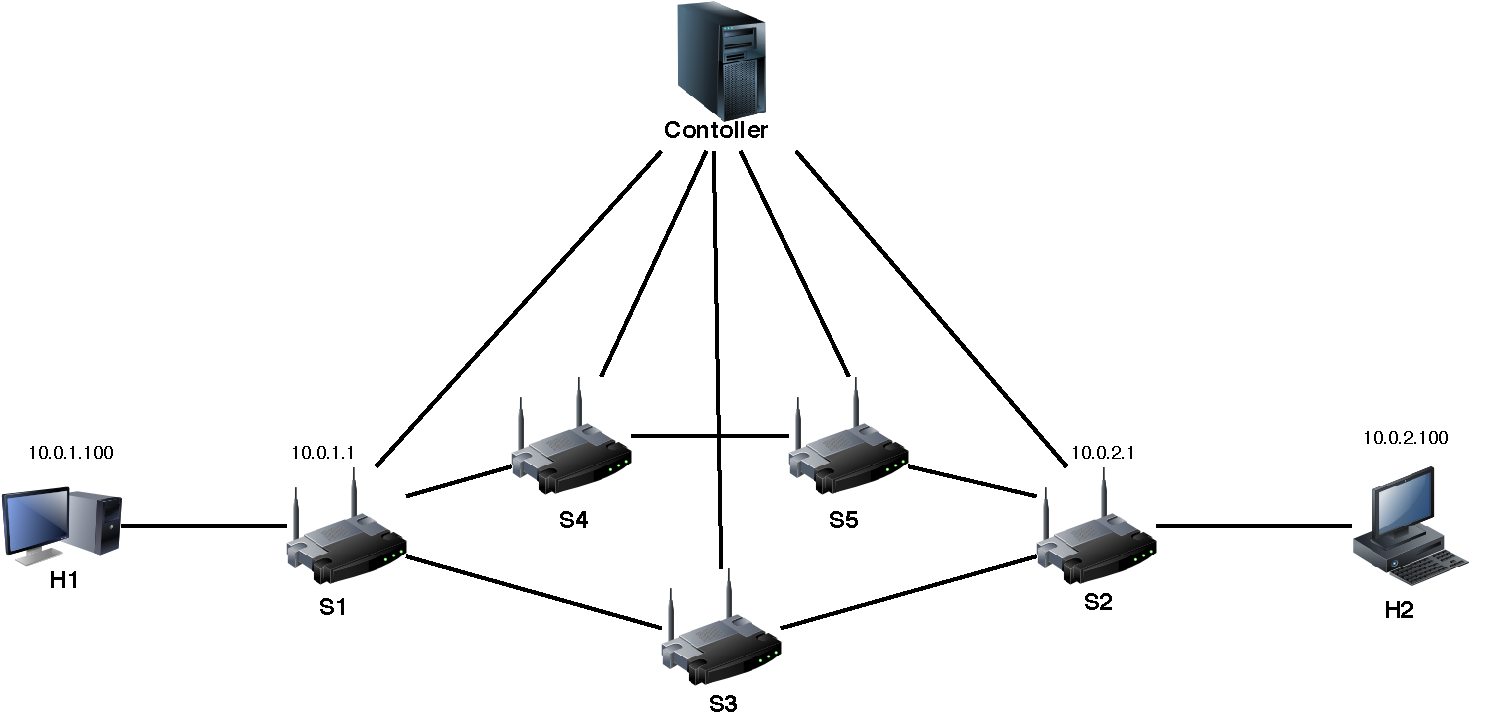
\includegraphics[scale = 0.60]{../images/psik_topology_2.pdf}
		\caption{Schemat architektury rozwiązania}
		\label{f:arch}
	\end{figure}
	\subsection{Założenia}
	\begin{itemize}
		\item trasowanie: wybór najkrótszej ścieżki,
		\item metryka: liczba przeskoków,
		\item algorytm trasowania: wektor odległości (poprzednio algorytm Bellmana-Forda),
		\item przekazywanie tablic routingu z wykorzystaniem pakietów protokołu RIP,
		\item reaktywność: pierwsze pakiety wysyłane w sieci służą do określenia topologii i nie są przekazywane (brak konieczności generowania niepotrzebnego ruchu sieciowego kosztem utraty części pakietów),
	\end{itemize}
	
	\subsection{Implementacja}	
	Z każdym nowo-odkrytym urządzeniem tworzony jest obiekt klasy \texttt{Switch}, z którym powiązana jest tablica routingu, jak również słowniki zapisujące relacje między portami, adresami MAC dostępnych pod nimi urządzeń oraz ich adresy IP. Co 2 sek. kontroler rozsyła do wszystkich podłączonych routerów aktualne tablice routingu (RIP Response) wraz z regułą wysłania jej do wszystkich sąsiadów routera. Przy każdym wysłaniu dekrementowany jest czas życia rekordu tablicy routingu. Podsieć jest usuwana po upływie związanego z nią czasu ważności rekordu.
	
	Kontroler, po otrzymaniu tablicy routingu od routera, porównuje wartość metryki z aktualnie przypisaną wartością i, jeśli nowa wartość jest mniejsza (ścieżka zawiera mniej przeskoków) rekord tablicy jest aktualizowany.
	
	Zapytania wysyłane do kontrolera w odpowiedzi na otrzymane przez router pakiety RIP wykorzystywane są dodatkowo do określenia zależności pomiędzy portem routera a adresem fizycznym dostępnym z tego portu. Zarówno ta informacja jak i dane o dostępnych podsieciach są również aktualizowane po otrzymaniu pakietu ARP. Mając informacje o dostępnych podsieciach możliwe jest instalowanie przepływu pakietów na odpowiedni port.
	\subsection{Opis reprezentatywnych reguł zapisywanych w tablicach przepływów przełączników}
	
	\section{Demonstracja rezultatów (procedura testowania)}
	W~ramach przedstawienia poprawności implementacji wyłączany będzie jeden z~routerów nie połączony z~hostem. Następnie zaprezentowany będzie przesył informacji z~jednego hosta do drugiego z~wykorzystaniem alternatywnej trasy. 
	\subsection{Cel częściowy}
	W ramach odbioru częściowego zaprezentowano implementację połączonej zgodnie z rysunkiem emulowanej sieci oraz następujące funkcje: odkrywanie topologii sieci, umożliwienie komunikacji między urządzeniami oraz wybór najkrótszej ścieżki.
	\subsection{Testowanie wersji finalnej}
%	Zaprezentowanie poprawnego działania sieci jest możliwe 
	Testy działania projektu wykonano poprzez uruchomienie emulatora sieci i kontrolera - dla jej domyślnego ustawienia ruch kierowany jest najkrótszą ścieżką, a więc przez router \texttt{s3}. Po odłączeniu tego routera (\verb|switch s3 stop|) ruch kierowany jest po kolejnej najkrótszej dostępnej ścieżce, a więc przez routery \texttt{s4} i \texttt{s}. Analogicznie, po pojawieniu się nowego routera (lub przywróceniu dawniej wyłączonego \texttt{s3} (\verb|switch s3 start|)) ruch sieciowy kierowany jest po najlepszej ścieżce.
	
	Informacje na temat wybranej ścieżki są wyświetlane na standardowym wyjściu przez program kontrolera.
	
%	W~trakcie odbioru częściowego planowane jest pokazanie zaimplementowanej sieci, połączonej zgodnie z~rysunkiem \ref{f:arch}, w~której przesył danych pomiędzy hostami następuje po podstawowej ścieżce. 

	\section{Wykaz załączonych plików źródłowych.}
	\begin{itemize}
		\item \textbf{router1.py} : plik kontrolera \\ 
		\verb|./pox.py log.level --DEBUG router1 samples.pretty_log openflow.discovery|
		\item \textbf{mytopo\_test.py} : topologia sieci \\
		\verb|sudo mn --custom mytopo_test.py --topo mytopo --mac --switch ovsk --controller remote|%,ip=192.168.56.1,port=6633|
	\end{itemize}
	
%	\section{Podział prac}
%	Tabela \ref{t:podzial_prac} przedstawia ustalony podział pracy w~zespole.
%	\begin{table}[h]
%		\centering
%		\begin{tabular}{|c|c|c|}
%			%\begin{tabular}{|m{1.5em}|m{17 em}|m{16em}|}
%			\hline
%			osoba& Kamila Lis & Karolina Borkowska\\
%			\hline
%			zadania & implementacja sterownika& przygotowanie symulacji sieci\\
%			\hline
%		\end{tabular}	
%		\caption{Podział prac w zespole}
%		\label{t:podzial_prac}
%	\end{table}
	
	

	
\end{document}